\documentclass{article}
\usepackage{bookmark}

\usepackage[utf8]{inputenc}
\usepackage[brazil]{babel}  % Define o idioma para português do Brasil
\usepackage{csquotes}       % Para lidar com aspas de maneira apropriada com babel
\usepackage{array}
\usepackage{amsmath}
\usepackage{xcolor}

\usepackage{amsmath}
\usepackage{xcolor}
\usepackage{listings}
% Configuração do estilo de código
\lstset{
  language=C,
  %basicstyle=\ttfamily\footnotesize,
  keywordstyle=\color{blue},
  commentstyle=\color{gray},
  stringstyle=\color{red},
  breaklines=true,
  frame=single,
  numbers=left,
  numberstyle=\tiny,
  numbersep=5pt,
  showstringspaces=false,
}


\usepackage{graphicx}       % Pacote para inserção de imagens

\usepackage{hyperref}       % Pacote para links clicáveis
\hypersetup{
    colorlinks=true,
    linkcolor=blue,
    urlcolor=blue,
}

\usepackage{enumitem}       % Pacote para personalização de listas

\usepackage{geometry}       % Pacote para ajustar margens

\geometry{                  % Definindo margens personalizadas (em centímetros)
  left=2.5cm,  % Margem esquerda
  right=2.5cm, % Margem direita
  top=2.5cm,   % Margem superior
  bottom=2.5cm % Margem inferior
}

\usepackage[backend=biber,style=ieee]{biblatex}     % Estilo ieee para bibliografia numerada
\addbibresource{ref.bib}                            % Arquivo .bib


\begin{document}

\begin{titlepage}
    \centering
    % Cabeçalho personalizado
    
\includegraphics[width=0.3\textwidth]{../../Topic1/Avaliativo/Imagens/Logo UFLA - Colorida chapada.png}

    \vspace*{2cm} % Espaçamento vertical antes do cabeçalho
    \Large
    Universidade Federal de Lavras\\
    PPGCC\\
    PCC508 – Sistemas Operacionais\\
    
    \vspace{2cm} % Espaço entre o cabeçalho e o título
    \huge % Define o tamanho da fonte do título
    \textbf{Tópico 10 Lista Avaliativa}
    
    \vfill % Adiciona um espaçamento flexível antes do rodapé (opcional)
    
    % Opcionalmente, você pode incluir seu nome e a data aqui
    \large
    Douglas Aquino T. Mendes\\
    \today % Insere a data atual
\end{titlepage}

\tableofcontents
\newpage

\section{Introdução}
Este documento tem como objetivo apresentar o desenvolvimento das atividades avaliativas para o tópico 10 da disciplina de Sistemas Operacionais, focando na implementação de códigos em linguagem C. Serão apresentadas as questões, a resolução, os códigos desenvolvidos, seguido da apresentação dos resultados da execução do código.

\section{Questões}

\subsection{1}
\textbf{Pergunta:} 1) O Kernel pode ser considerado um extenso executável que recebe solicitações dos programas em execução e é responsável por lidar com elas, além de fazer o gerenciamento de recursos. Explique em quais partes podem ser divididas as funções do Kernel.\newline

\textbf{Resposta:}  O kernel atua como uma ponte entre o hardware e o software, oferecendo uma camada de abstração para os programas de usuário. Ele é responsável por duas funções principais: fornecer aos programadores de aplicativos um conjunto limpo de recursos abstratos e gerenciar os recursos de hardware \parencite[p. 2]{tanenbaum2021}. As funções do kernel podem ser divididas em várias partes:

\begin{itemize}
  \item Gerenciamento de processos: O kernel cria, gerencia e finaliza processos \parencite[p. 506]{tanenbaum2021}.
  \item Gerenciamento de memória: O kernel gerencia a memória principal do computador, incluindo a alocação, proteção e mapeamento de endereços de memória para os processos \parencite[p. 233]{tanenbaum2021}.
  \item Gerenciamento de entrada e saída (E/S): O kernel interage com os dispositivos de E/S, emitindo comandos para eles, interceptando interrupções e lidando com erros.
  \item Comunicação entre processos (IPC): O kernel fornece mecanismos para que os processos possam se comunicar e sincronizar uns com os outros \parencite[p. 604]{tanenbaum2021}.
  \item Chamadas de sistema: O kernel fornece uma interface para que os programas de usuário possam solicitar serviços do sistema operacional, através de chamadas de sistema \parencite[p. 16]{tanenbaum2021}..
\end{itemize}

\section{Desenvolvimento de Códigos}

\subsection{2}

\textbf{Enunciado:} 2)  O Linux guarda a lista de todos os processos do sistema em uma lista circular. Cada elemento da lista é do tipo struct task\_struct que contém informações sobre o processo. O primeiro módulo de kernel que deve ser criado desta lista deve percorrer a lista de processos do kernel imprimindo informações sobre cada processo.\newline

\subsubsection{Código}
\label{sub-sec-cod1}
\lstinputlisting[language=C]{Codes/atv2/list_processes.c}

\subsubsection{Testes e Resultados}
Como resultado da execução do código exibido na subceção \ref{sub-sec-cod1}, obtivemos a saída ilustrada na figura \ref{fig:exec1}. 

\begin{figure}[ht]
    \centering
    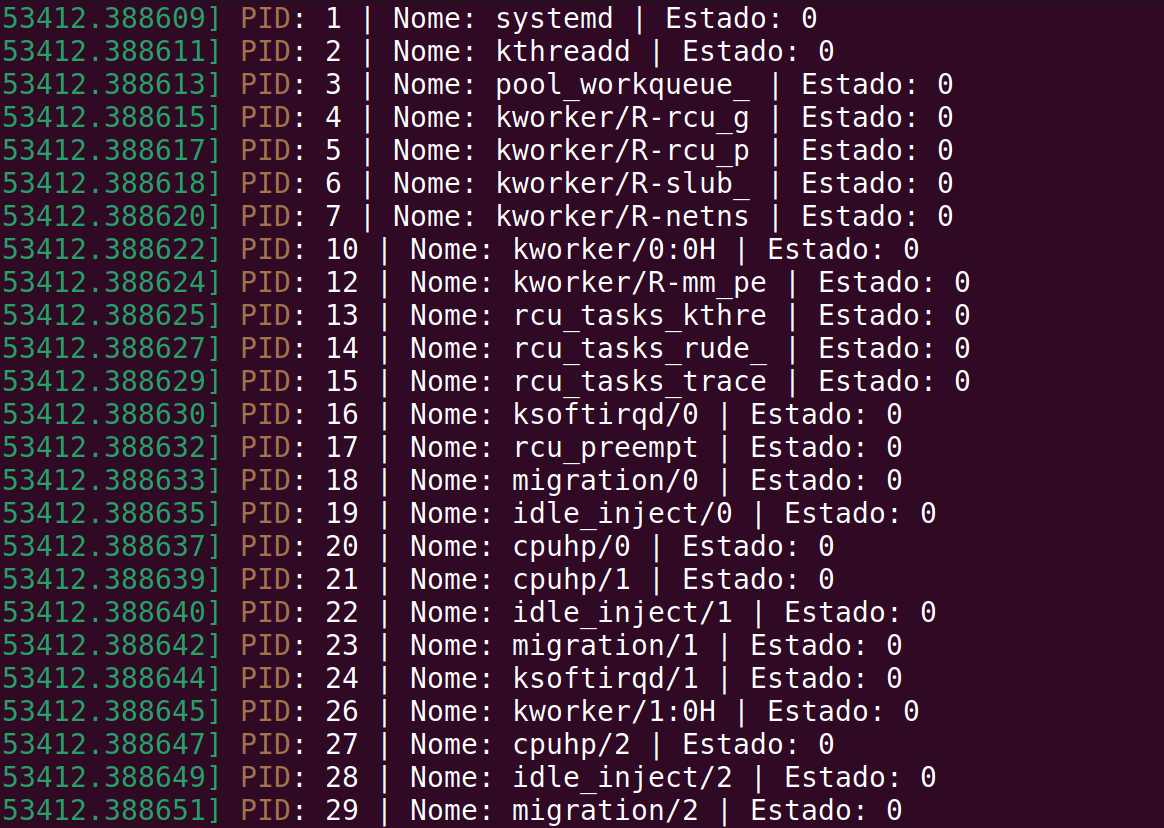
\includegraphics[width=1\textwidth]{./Images/saida1.png}
    \caption{Resultado da execução do programa}
    \label{fig:exec1}
\end{figure}


\subsection{3}

\textbf{Enunciado:} 3) Esse exercício é continuação de um feito na lista de estudo. Desenvolva um módulo de Kernel do Linux que seja um driver de dispositivo do tipo caractere. Cada vez que um dado é escrito no Driver, ele deve ser guardado em uma lista do kernel criada para isso. No caso
de leitura, cada leitura deve retirar um nó dessa lista e retornar os dados. Se a lista estiver vazia, deve retornar a palavra “vazia”.\newline

\subsubsection{Código}
\label{sub-sec-cod1}
\lstinputlisting[language=C]{Codes/atv3/mod3.c}

\subsubsection{Testes e Resultados}
Como resultado da execução do código exibido na subceção \ref{sub-sec-cod1}, obtivemos a saída ilustrada na figura \ref{fig:exec2}. 

\begin{figure}[ht]
  \centering
  \begin{minipage}{0.45\textwidth}
      \centering
      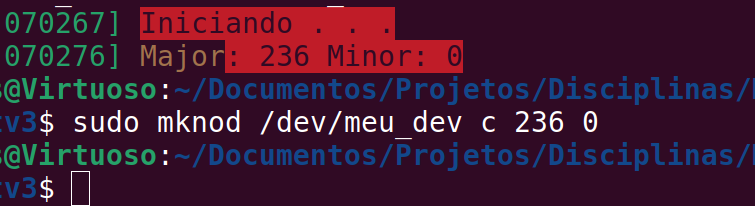
\includegraphics[width=\textwidth]{Images/atv2-1.png}
      \caption{Criando o dispositivo}
      \label{fig:imagem1}
  \end{minipage}\hfill
  \begin{minipage}{0.45\textwidth}
      \centering
      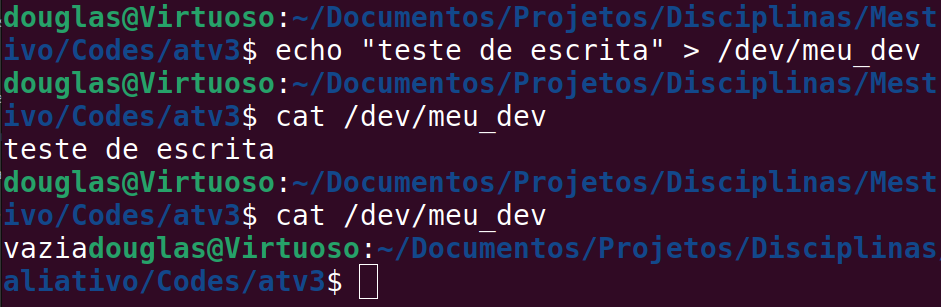
\includegraphics[width=\textwidth]{Images/atv22.png}
      \caption{Escrevendo e lendo do dispositivo}
      \label{fig:imagem2}
  \end{minipage}
  \caption{Modulo instalado e Teste do dispositivo}
  \label{fig:exec2}
\end{figure}

\printbibliography % Imprime a lista de referências


\end{document}